\ifx\allfiles\undefined
\input{00_prefix}%前缀
\begin{document}
\else
\fi
%分文件开始


\begin{center}
	\begin{table}[H]  %table 里面也可以嵌套tabular,只有tabular是不能加标题的
		\centering
		\caption{模型特征概要}  %表格标题
		\resizebox{200pt}{75pt}{
			\begin{tabular}{cc}
				\hline
				特征名称     & 权重   \\
				\hline
				守约评分     & 0.5972 \\
				经营规模评价 & 0.1413 \\
				经营利润率   & 0.0722 \\
				供应侧稳定性 & 0.0609 \\
				需求侧稳定性 & 0.1284 \\
				\hline
			\end{tabular}}
	\end{table}
\end{center}



我们得到的测试集数据预览结果如图所示:\begin{center}
	\begin{table}[H]  %table 里面也可以嵌套tabular,只有tabular是不能加标题的
		\centering
		\caption{测试集数据预览}  %表格标题
		\resizebox{200pt}{50pt}{
			\begin{tabular}{cccrrrr}
				\hline
				预测结果Y & 信誉评分 & 守约评分 & 经营规模评价 & 经营利润率 & 供应侧稳定性 & 需求侧稳定性 \\
				\hline
				2.00      & 2        & 1        & 0.0000       & 27.9825    & 1.0000       & 0.7470       \\
				3.00      & 4        & 1        & 0.0012       & 1.4693     & 0.9815       & 0.8815       \\
				1.00      & 1        & 0        & 0.0001       & -0.8618    & 0.9534       & 0.8362       \\
				1.00      & 1        & 0        & 0.0001       & 24.7661    & 1.0000       & 0.6970       \\
				2.50      & 3        & 1        & 0.0002       & 19.7709    & 1.0000       & 0.9508       \\
				1.00      & 1        & 0        & 0.0000       & -0.5566    & 0.9079       & 0.8667       \\
				1.50      & 1        & 0        & 0.0007       & 0.6984     & 0.9683       & 0.9708       \\
				3.67      & 3        & 1        & 0.0109       & 11.6644    & 0.9904       & 0.8442       \\
				3.50      & 3        & 1        & 0.0010       & 2.7676     & 0.9771       & 0.9061       \\
				3.00      & 3        & 1        & 0.0121       & 7.3478     & 0.9231       & 0.9227       \\
				\hline
			\end{tabular}}
	\end{table}
\end{center}



\begin{table}[htbp]  %table 里面也可以嵌套tabular,只有tabular是不能加标题的
	\centering
	\caption{工程参数}  %表格标题

	\resizebox{400pt}{150pt}{
		\begin{tabular}{cc}

			\hline
			参数名                           & 参数值 \\
			\hline
			数据切分                         & 0.75   \\
			数据洗牌                         & 是     \\
			交叉验证                         & 否     \\
			随机种子                         & 0      \\
			分裂准则                         & mse    \\
			树的最大深度                     & None   \\
			分裂节点时的策略                 & best   \\
			分裂一个内部节点所需最少样本数   & 2      \\
			每个叶子节点所需最少样本数       & 2      \\
			叶子节点中样本的最小权重         & 0      \\
			搜寻最佳划分的时候考虑的特征数量 & None   \\
			叶子节点的最大数量               & None   \\
			信息墒或者基尼系数不纯度的阀值   & 0      \\
			\hline
		\end{tabular}
	}
	\begin{figure}[H]
		\centering
		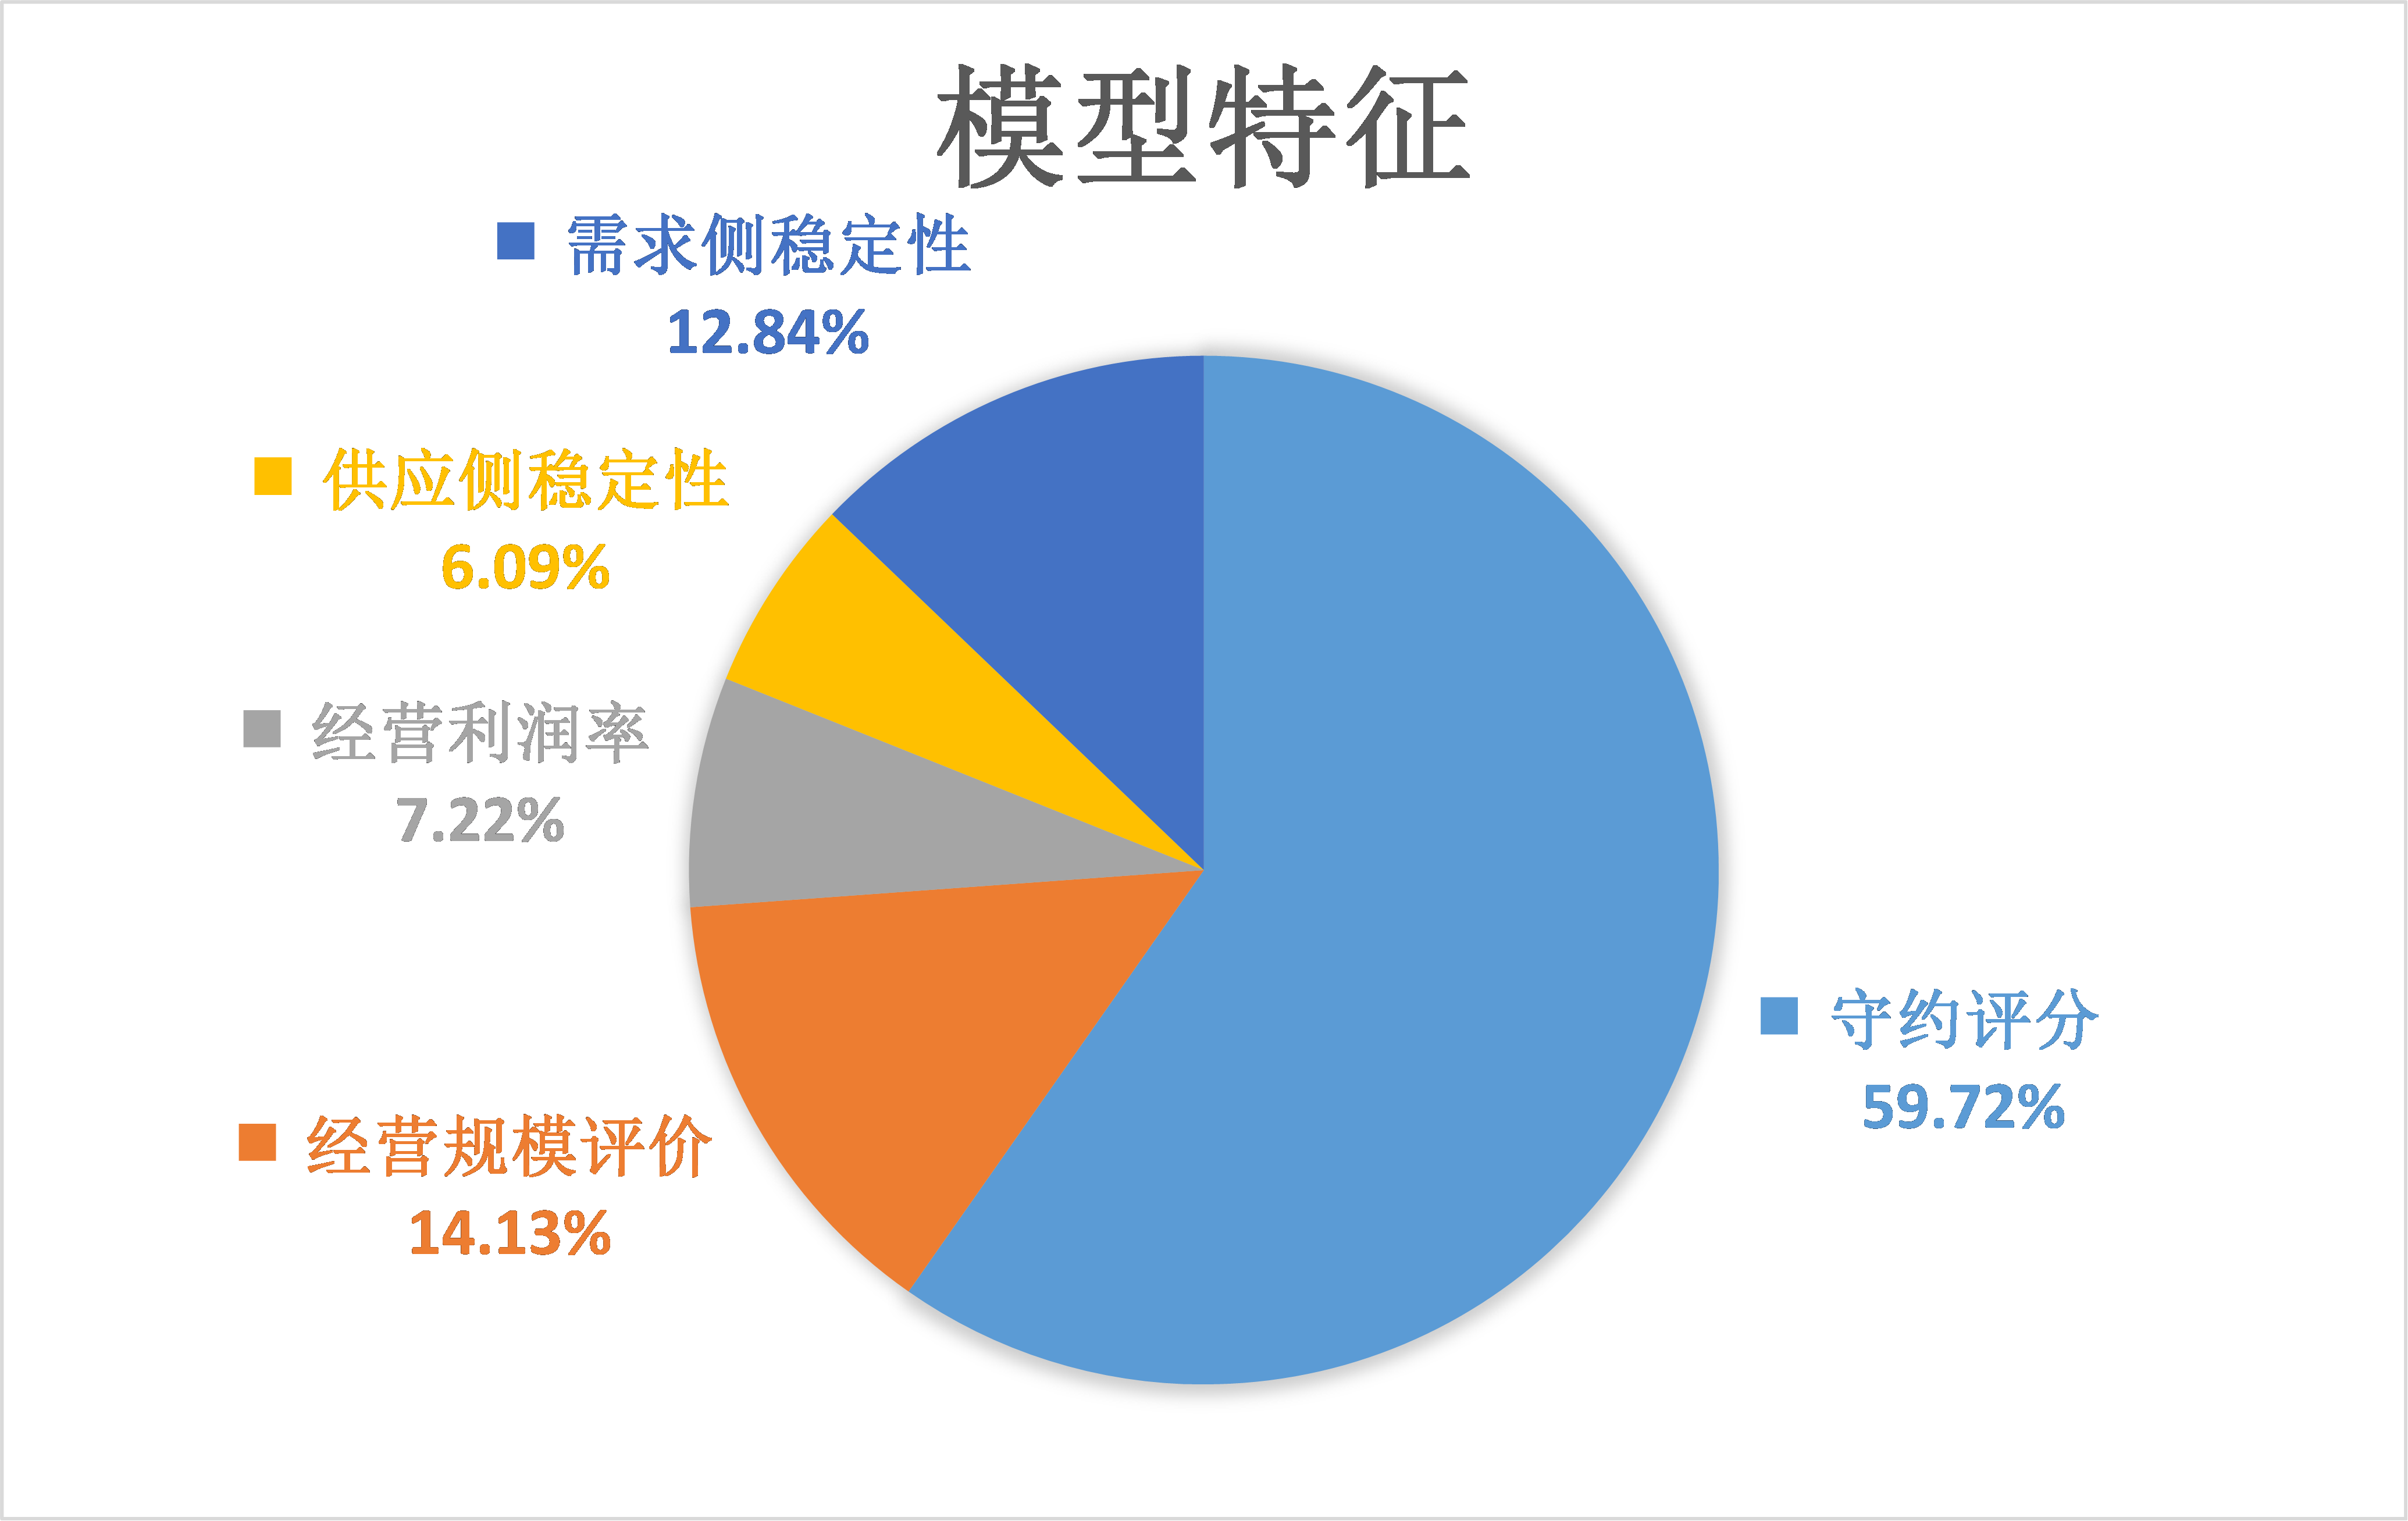
\includegraphics[width=0.75\linewidth]{figure/q2ModelAnalysis}%宽度，源文件相对位置
		\caption{模型特征}%图片下方的标题
		\label{fig:q2ModelAnalysis}%图片引用时所需标签
	\end{figure}
\end{table}

%分文件结束
\ifx\allfiles\undefined
\end{document}
\fi